\documentclass[11pt,letterpaper]{article}
\usepackage{array}
\usepackage{fullpage}
\usepackage{verbatim}
\usepackage{parskip}
\usepackage{graphicx}
\usepackage{url}
	\usepackage{xcolor,colortbl}
	\definecolor{gray}{rgb}{0.95,0.95,0.95}
	\newcommand{\gray}{\cellcolor{gray}}  %{0.9}
\usepackage[flushmargin]{footmisc}

%%%%%%%%%%%%%%%%%%%%%%%%%%%%%%%%%%%%%%%%%%%%
\usepackage{termcal}
% Few useful commands (our classes always meet either on Monday and Wednesday 
% or on Tuesday and Thursday)

\newcommand{\MTWFClass}{%
\calday[Monday]{\classday} % Monday
\calday[Tuesday]{\classday} % Tuesday
\calday[Wednesday]{\classday} % Wednesday
\skipday % Thursday (no class)
\calday[Friday]{\classday} % Friday 
\skipday\skipday % weekend (no class)
}

\newcommand{\holiday}[2]{%
\options{#1}{\noclassday}
\caltext{#1}{#2}
}

\newcommand{\lab}[2]{%
\options{#1}{\noclassday}
\caltext{#1}{#2}
}


\renewcommand{\calprintdate}{%
     \ifnewmonth\framebox{\arabic{month}/\arabic{date}}%
     \else\arabic{month}/\arabic{date}%
     \fi}
         
%%%%%%%%%%%%%%%%%%%%%%%%%%%%%%%%%%%%%%%%%%%%
\renewcommand{\thefootnote}{\fnsymbol{footnote}}

\newcommand{\squeezeup}{\vspace{-2.5mm}}
\setlength{\parindent}{0in}
\newcommand{\tablespace}[0]{\vspace{8pt}}

\begin{document}
\begin{centering}
\textbf{PHYS S211: General Physics I}

Fall 2024\\
\hfill{}\\

\bigskip
\begin{table}[h]
\centering
\setlength{\extrarowheight}{2pt}
\squeezeup
\begin{tabular}{@{}r@{\hspace{0.1in}}p{4.25in}} 
{\bf Instructor:} & Jason Amundson\\
& {\'A}ak'w T{\'a} H{\'i}t 209 \\
& jmamundson@alaska.edu\\
& phone: 796-6247 \tablespace\\
{\bf Class hours:} & MWF 10:45 am -- 11:45 am \tablespace\\
{\bf Lab hours:} & J01, T 8:45 am -- 11:45 am\\
& J02, T 1:15 pm -- 4:15 pm \tablespace\\
{\bf Office hours:} & MW 12:00 pm -- 1:00 pm, or by appointment\tablespace\\
{\bf Website:} & A course website will be maintained on Blackboard (http://classes.alaska.edu). Check for assignments, handouts, grades, and messages.\tablespace\\
{\bf Prerequisites:} & MATH S251\tablespace\\
{\bf Textbook:} & Physics for Scientists and Engineers: A Strategic Approach with Modern Physics (5\textsuperscript{th} ed.) by Knight. Be sure to purchase a version of the book that comes with an access card for MasteringPhysics, which you will use for homework submissions.
\tablespace\\
& The cheapest option, which is available through the MBS page, is to purchase the MasteringPhysics with Pearson eText package (ISBN-13: 978-0-13-680847-3).
\tablespace\\
& To access MasteringPhysics, follow the link from the course Blackboard site and click ``Open MyLab and Mastering''. From there you will need to enter the access code that you received when you purchased the textbook.  \tablespace\\
{\bf Other materials:} & A basic, simple scientific calculator with trigonometric, exponential, and logarithmic functions. Calculators can be used during exams.
\end{tabular}
\end{table}
\end{centering}

\textbf{Student Learning Outcomes}\\
Upon successful completion of this course, students will be able to:
\begin{enumerate}\itemsep -5pt
\item Describe basic physics principles, including motion, energy, waves, and thermodynamics
\item Solve analytical problems using calculus and basic physics principles
\item Test basic physics principles through experimentation and computer analysis of laboratory data
\end{enumerate}\bigskip

\clearpage
Physics is the study of matter and its motion through space and time. In PHYS S211 we will cover the field of classical mechanics, which pertains to ``large'' objects that are moving much slower than the speed of light.

\bigskip
\
\begin{figure}[h]
\begin{center}
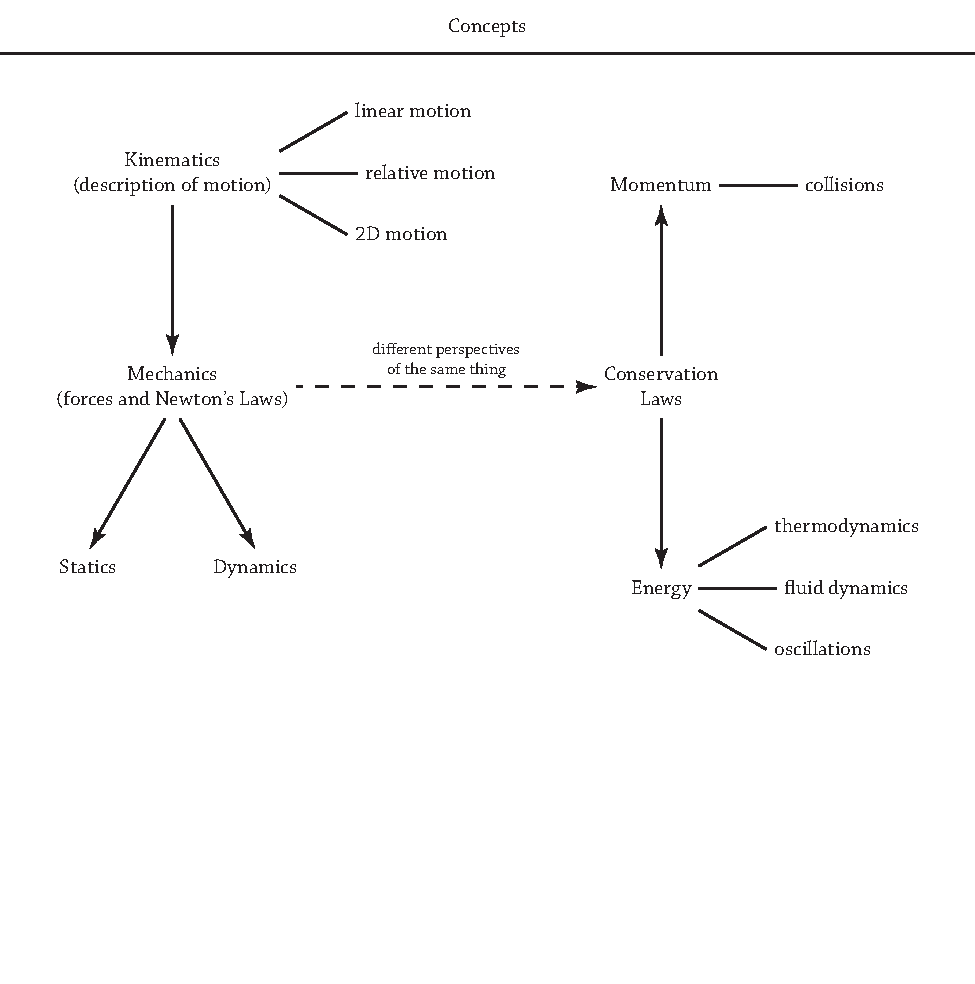
\includegraphics[width=6.5in]{./flowchart.pdf}
\end{center}
\end{figure}

\clearpage
\textbf{Grading} 
\begin{table}[h!]
\squeezeup
\begin{tabular}{ll}
Homework assignments & 20\%\\
Informal lab reports (8) & 20\%\\
Formal lab reports (2) & 15\%\\
Exams (3) & 45\%
\end{tabular}
\end{table}

\textbf{Homework}\\
There will be 10 homework assignments consisting of roughly 10 problems each. You will submit your solutions through MasteringPhysics. Late assignments will only be accepted for extenuating circumstances.

Why use MasteringPhysics?
\begin{itemize}\itemsep -5pt
\item It gives you wrong-answer feedback and hints for solving problems.
\item It provides me with diagnostics on what types of problems are giving you the most trouble.
\item The ``study area'' includes some nice material that complements what we will discuss in class and labs.
\end{itemize}

A few suggestions for working through the homework:
\begin{itemize}\itemsep -5pt
\item Work through your answers slowly and be sure to check for significant figures before entering your solution. You might consider solving all of the problems before entering your answers so that you don't get frustrated right away.
\item If you feel confident in your answer, but MasteringPhysics tells you that your answer is incorrect and doesn't give you useful feedback, send me an e-mail. View this as an opportunity to figure out what you did wrong and correct your mistake before the due date.%, which is an option that you wouldn't have with paper submission.
\item I view the homework as training for the exams, and in that sense the homework grade is essentially participation. I'm happy to help you work through problems all the way to the final solution if you are having trouble. 
\item I reserve time in class each week to address questions related to the homework, so come with questions!
\end{itemize}

\textbf{Lab reports}\\
There will also be 10 laboratory exercises during the semester. You will be expected to turn in informal reports for eight of the labs and formal reports for the other two. For the informal reports you may submit a group report (no more than three people in a group) but are not required to do so. For the formal reports I expect you to submit an individual report. More details to follow. You may submit physical or electronic copies of your reports; if you choose to submit a report electronically you should do so by uploading it to Blackboard.

Lab reports will not be considered late up until the point that I grade them; afterwards they will be docked by 50\%. This late policy is designed to (1) encourage you to finish your reports even if they were not completed before the due date and (2) simplify my grading. I don't like taking off points for late work, especially if I am slow at grading it, but it is also much easier to grade everybody's work at once. I think this policy is a good compromise. 
\\

\textbf{Exams}\\
You will be given three exams during the semester, including the final exam. The exams will focus on the material that was covered over the previous third of the semester, but they are cumulative in the sense that everything that we do in physics will be built up from the same core principles. The exams will be proctored in the Learning Center. You will have several days to complete them. The exam scores will be curved.\\

%\clearpage
\textbf{Grading Scale}
\begin{table}[h!]
\squeezeup
\begin{tabular}{ll}
A & 93--100\% \\
A- & 90--92\% \\
B+ & 87--89\% \\
B & 83--86\% \\
B- & 80--82\% \\
C+ & 77--79\% \\
C & 73--76\% \\
C- & 70--72\% \\
D+ & 67--69\% \\
D & 63--66\% \\
D- & 60--62\% \\
F & $<$60\%
\end{tabular}
\end{table}

%I may lower this grading scale if I decide that the course assignments have been too difficult. I will not do the opposite. \\

%\textbf{General Comments}\\
%My job is to help you learn. If you are uncomfortable in the classroom or have any other comments and concerns, please do not hesitate to contact me.

%When I'm in the office I'll try to respond to your phone calls and e-mails as quickly as possible. However, in general I do not respond to messages after 6:00 pm or on weekends. Any messages sent to me during that time might not be addressed until the following morning.\\

%\textbf{Conduct}\\
%Please turn off cell phones, laptops, and other electronic devices (except calculators) during lecture. They can be a distraction to you and your fellow students.\\

\textbf{Student Ratings of Instruction}\\
During the last three weeks of class, you will have an opportunity to complete an online rating questionnaire on course instruction, how the course aided in your skill development,  effectiveness of technology and equipment used, and adequacy of library resources and services used during the course. You will receive notification in your UAS email account when the rating questionnaire is available. Please make use of this opportunity to provide feedback on what worked for you and what did not. Your input is used to assess methods and services in order to provide the best educational experience possible.\\

\textbf{Disabilities}\\
If you experience a disability and would like information about support services, please contact Disability Services, located at the Student Resource Center in the Mourant building.  They can be reached at 796-6000. For more information, please see http://www.uas.alaska.edu/dss/index.html.\\

\textbf{Title IX/Sexual Misconduct}\\
All students have the right to be free from all forms of gender and sex-based misconduct (sexual harassment, dating violence, domestic violence, sexual assault, or stalking). Please report any incidence of sex or gender-based discrimination to the UAS Title IX Office: 796-6036 or email {title9@uas.alaska.edu}. More information and resources are available at\\ http://www.uas.alaska.edu/policies/titleix.html.

\clearpage
\textbf{Schedule (subject to change)}\\
I have one day of field work that I need to do during the fall that is very weather dependent. I may need to cancel one class at fairly short notice if it looks like there won't be many options for getting out to the field on days that I'm not teaching. 
\begin{center}
\begin{calendar}{8/26/2024}{16} % Semester starts on 8/27/2018 and lasts for 15
                    % weeks, including finals week
\setlength{\calboxdepth}{.6in}
\renewcommand{\calprintclass}{}
\MTWFClass

% August
\caltexton{1}{Course overview: why physics?}
\caltextnext{1.1--1.6: Introduction to kinematics}
\caltextnext{2.1--2.5: Kinematic equations}

% September
\caltextnext{\gray 4.1--4.2: Motion in two dimensions\\{\bf HW \#1 due}}

\caltextnext{\gray 4.3 Projectile motion}
\caltextnext{\gray 2.6: Motion on inclined planes}
\caltextnext{\gray 4.3: Relative motion}

\caltextnext{\gray 4.4--4.6, 12.1: Circular and rotational motion}
\caltextnext{\gray 5.1--5.7, 7.1--7.3: Newton's Laws}
\caltextnext{\gray 5.2, 6.3: Types of forces, I\\{\bf HW \#2 due}}

\caltextnext{\gray 6.4--6.5, 7.4: Types of forces, II}
\caltextnext{\gray 6.5, 9.4: Types of forces, III}
\caltextnext{\gray 8.2--8.4: Centripetal force\\{\bf HW \#3 due}}
\caltextnext{\gray {\bf Exam \#1}\\No class}
\caltextnext{\gray 12.5--12.7: Torque}

% October
\caltextnext{12.5--12.7: Torque, II}
\caltextnext{12.8 Static equilibrium}
\caltextnext{14.6: Equilibrium and elasticity}
\caltextnext{11.1: Impulse and momentum \\{\bf HW \#4 due}}

\caltextnext{11.2--11.5: Conservation of momentum }
\caltextnext{12.10: Vector description of torque\\{\bf HW \#5 due}}
\caltextnext{12.11: Angular momentum}

\caltextnext{9.1--9.3: Introduction to energy}
\caltextnext{9.1--9.3: Work and energy\\{\bf HW\#6 due}}
\caltextnext{10.1--10.8: Work and energy, II}


% November
\caltextnext{10.1--10.8: Work and energy, III }
\caltextnext{19.1, 19.4: Introduction to thermodynamics\\{\bf HW \#7 due} }
\caltextnext{\gray {\bf Exam \#2}\\No class}

\caltextnext{\gray 19.5--19.6: Latent and specific heat}
\caltextnext{\gray 19.8: Heat transfer}

\caltextnext{\gray 18.6--18.7, 19.2, 19.7: Thermodynamics of gases}
\caltextnext{\gray 14.1--14.3: Introduction to fluids}
\caltextnext{\gray 14.4: Archimedes' principle\\{\bf HW \#8 due}}

\caltextnext{\gray 14.5: Fluid dynamics, I}
\caltextnext{\gray 14.5: Fluid dynamics, II}
\caltextnext{\gray 15.1--15.6: Oscillations \\{\bf HW \#9 due}}

\caltextnext{\gray 15.7--15.8: Driven and damped oscillations}
\caltextnext{\gray 16.1--16.2: Introduction to waves}

% December
\caltextnext{16.3: Traveling waves}

\caltextnext{17.1--17.8: Wave superposition and sound}
\caltextnext{Course summary\\{\bf HW \#10 due}}

% Labs

\lab{8/27/2024}{No lab}
\lab{9/3/2024}{\gray Lab \#1: Measurements and motion}
\lab{9/10/2024}{\gray Lab \#2: Acceleration\\{\bf Lab \#1 due}}
\lab{9/17/2024}{\gray Lab \#3: Forces\\{\bf Lab \#2 due}}
\lab{9/24/2024}{\gray Review for exam \#1\\{\bf Lab \#3 due}}

\lab{10/1/2024}{Lab \#4: Circular motion (formal report)}
\lab{10/8/2024}{Lab \#5: Torque \\{\bf Lab \#4 due}}
\lab{10/15/2024}{Lab \#6: Statics \\{\bf Lab \#5 due}}
\lab{10/22/2024}{Lab \#7: Momentum and energy\\{\bf Lab \#6 due}}
\lab{10/29/2024}{Review for exam \#2\\{\bf Lab \#7 due}}

\lab{11/5/2024}{\gray Lab \#8: Springs (formal report)}
\lab{11/12/2024}{\gray No lab}
\lab{11/19/2024}{\gray Lab \#9: Pendulums\\{\bf Lab \#8 due}}
\lab{11/26/2024}{\gray Lab \#10: Sound\\{\bf Lab \#9 due}}

\lab{12/3/2024}{Review for exam \#3\\{\bf Lab \#10 due}}

\holiday{9/2/2024}{\gray No class}
\holiday{10/11/2024}{No class}
\holiday{11/27/2024}{\gray No class\\Fall break}
\holiday{11/29/2024}{\gray No class\\Fall break}
\holiday{12/9/2024}{Final exam week - - -}
\holiday{12/10/2024}{- - - - - - - - - - - - - - -}
\holiday{12/11/2024}{- - - - - - - - - - - - - - -}
\holiday{12/13/2024}{- - - - - - - - - - - - - - $>$}

% Holidays
\holiday{9/5/2022}{\gray Labor Day}
\holiday{11/27/2020}{\gray Thanksgiving holiday}



\end{calendar}
\end{center}


\end{document}
